\begin{corrige}{DS2012-2-0001}

\begin{enumerate}  
  \item La fonction $\cos(x)+x^2$ est paire car elle est la somme de deux fonctions paires. La seule fonction qui est paire et impaire en m\^eme temps est la fonction nulle, donc $\cos(x)+x^2$ n'est pas impaire. 

    Cette fonction n'est pas p\'eriodique non plus : si elle l'\'etait il y aurait $T> 0$ tel que $\cos(x+T)+(x+T)^2 = \cos(x)+x^2$ pour tout $x$ dans $\eR$. Cela voudrait dire que  $\cos(T)+T^2 = 1$ (on prend $x=0$), $\cos(2T)+4T^2=\cos(T)+T^2$ (on prend $x= T$), et plus en générale, pour tout $k$ entier positif $ \cos(kT)+k^2T^2=1$. Cela n'est pas possible car $1-\cos(kT)$ est borné par $2$ alors que $k^2T^2$ peut devenir aussi grand qu'on veut quitte à prendre $k$ assez grand.   

  \item 
    \begin{figure}[ht!]
      \begin{center}
        \subfigure[ $f_1(x)=\cos(2x)$]{
          \label{f1}
          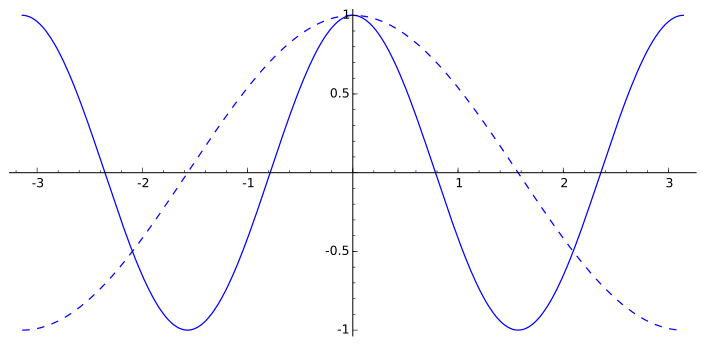
\includegraphics[width=4cm]{pictures_bitmap/cos2x.png}}
        \subfigure[ $f_2(x)=\frac{\cos(x)}{4}$]{
          \label{f2}
          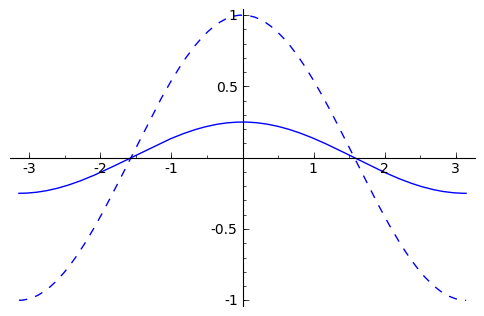
\includegraphics[width=4cm]{pictures_bitmap/quartcosx.png}}
        \subfigure[ $f_3(x)=\cos(x)-2$]{
          \label{f3}
          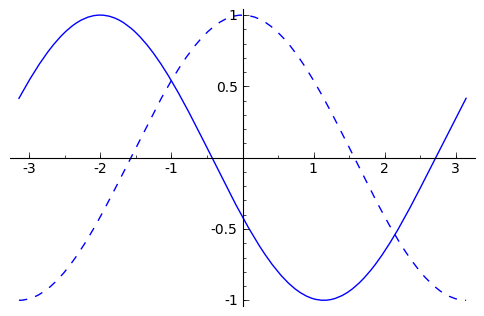
\includegraphics[width=4cm]{pictures_bitmap/cosxplus2.png}}
        \subfigure[ $f_4(x)=|\cos(x)|$]{
          \label{f5}
          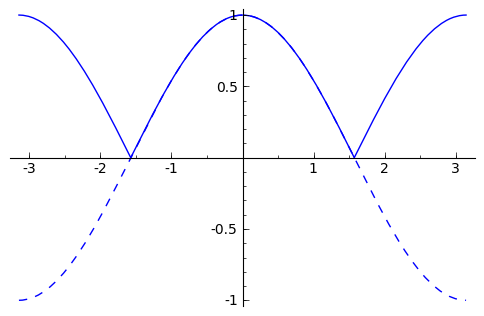
\includegraphics[width=4cm]{pictures_bitmap/abscosx.png}}
      \end{center}
      \caption{Les graphes des fonctions $f_1,\ldots, f_4$}
      
    \end{figure}
    
  \end{enumerate}
\end{corrige}
